We first review the conditions for which a local energy deposition in a WD results in runaway fusion.
Any energy deposit will eventually heat ions within some localized region---parameterize this region by its linear size $L_0$, total kinetic energy $\Ez$ and typical temperature $T_0$.
These scales evolve in time, but it will be useful to describe a given heating event by their initial values.

The fate of a heated region is either a nonviolent diffusion of the excess energy across the star, or a runaway fusion chain-reaction that destroys the star.
The precise outcome depends on $L_0$, $\Ez$ and $T_0$.
There is a critical temperature $T_f$, set by the energy required for ions to overcome their mutual Coulomb barrier, above which fusion occurs.
For carbon burning, $T_f \sim \MeV$~\cite{Gasques:2005ar}.
Any heated region $T_0 > T_f$ will initially support fusion, although this is not sufficient for runaway as cooling processes may rapidly lower the temperature below $T_f$.
This cooling will not occur if the corresponding timescale is larger than the timescale at which fusion releases energy.
Cooling in a WD is dominated by thermal diffusion, and the diffusion time increases as the size of the heated region.
However, the timescale for heating due to fusion is independent of region size.
Thus, for a region at temperature $\gtrsim T_f$, there is a critical size above which the heated region does not cool but instead initiates runaway.
For a region at the critical fusion temperature $T_f$, we call this critical size the \emph{trigger size} $\lambda_T$.
The value of $\lambda_T$ is highly dependent on density, and in a WD is set by the thermal diffusivity of either photons or degenerate electrons.
This critical length scale has been computed numerically in~\cite{Woosley} for a narrow range of WD densities and analytically scaled for other WD masses in~\cite{Graham:2015apa}.
As in~\cite{Graham:2015apa}, we will restrict our attention to carbon-oxygen WDs in the upper mass range $\sim 0.85 - 1.4 ~M_{\astrosun}$ (these will yield the most stringent constraints on DM).
This corresponds to a central number density of ions $n_\text{ion} \sim 10^{30} - 10^{32} ~\cm^{-3}$ and a trigger size of $\lambda_T \sim 10^{-3} - 10^{-5} ~\text{cm}$.

If a heated region is smaller than the trigger size, its thermal evolution is initially dominated by diffusion.
However, this will still result in runaway fusion if the temperature is of order $T_f$ by the time the region diffuses out to the trigger size.
For our purposes it is more natural to phrase this in terms of the total energy $\Ez$ deposited during a heating event.
Of course, the relation between energy $\Ez$ and temperature $T_0$ depends on the rate at which WD constituents---ions, electrons, and photons---thermalize with each other within the region size $L_0$.
Given that the different species thermalize rapidly, the excess energy required to raise the temperature to $T_f$ in a volume $V$ is given by a sum of their heat capacities
\begin{equation}
\label{eq:heatcapacity}
  \frac{\Ez}{V} \gtrsim \int_0^{T_f} dT (n_\text{ion} + n_e^{2/3} T + T^3),
\end{equation}
where $n_e$ is the number density of electrons.
Note that we use the heat capacity of a degenerate gas of electrons, since the Fermi energy $E_F \gtrsim \MeV$ for the densities we consider.
The minimum energy deposit necessary to trigger runaway fusion is simply
\begin{align}
\label{eq:Eboom}
\Eboom &\sim \lambda_T^3 (n_\text{ion} T_f + n_e^{2/3} T_f^2 + T_f^4) \\
&\approx 10^{16} - 10^{23} ~\GeV. \nonumber
\end{align}
$\Eboom$ varies with $\lambda_T$ over the range of WD densities and is plotted in Figure~\ref{fig:Eboom}.
Thus for a heating event characterized by its $L_0$, $\Ez$, and $T_0 \gtrsim T_f$, there is an \emph{ignition condition}:
\begin{align}
    \label{eq:energy_boom_condition}
    \Ez \gtrsim
    \Eboom \cdot \text{max}\left\{1, \frac{L_0}{\lambda_T}\right\}^3.
\end{align}
Any $\Ez$ satisfying this condition is minimized for $L_0$ less than the trigger size, where it is also independent of the precise value of $L_0$.
For broader deposits, the necessary energy is parametrically larger than $\Eboom$ by a volume ratio $(L_0/\lambda_T)^3$.
As a result, understanding the $L_0$ for different kinds of heating events in a WD is critical to determining whether or not they are capable of destroying the star.

\begin{figure}
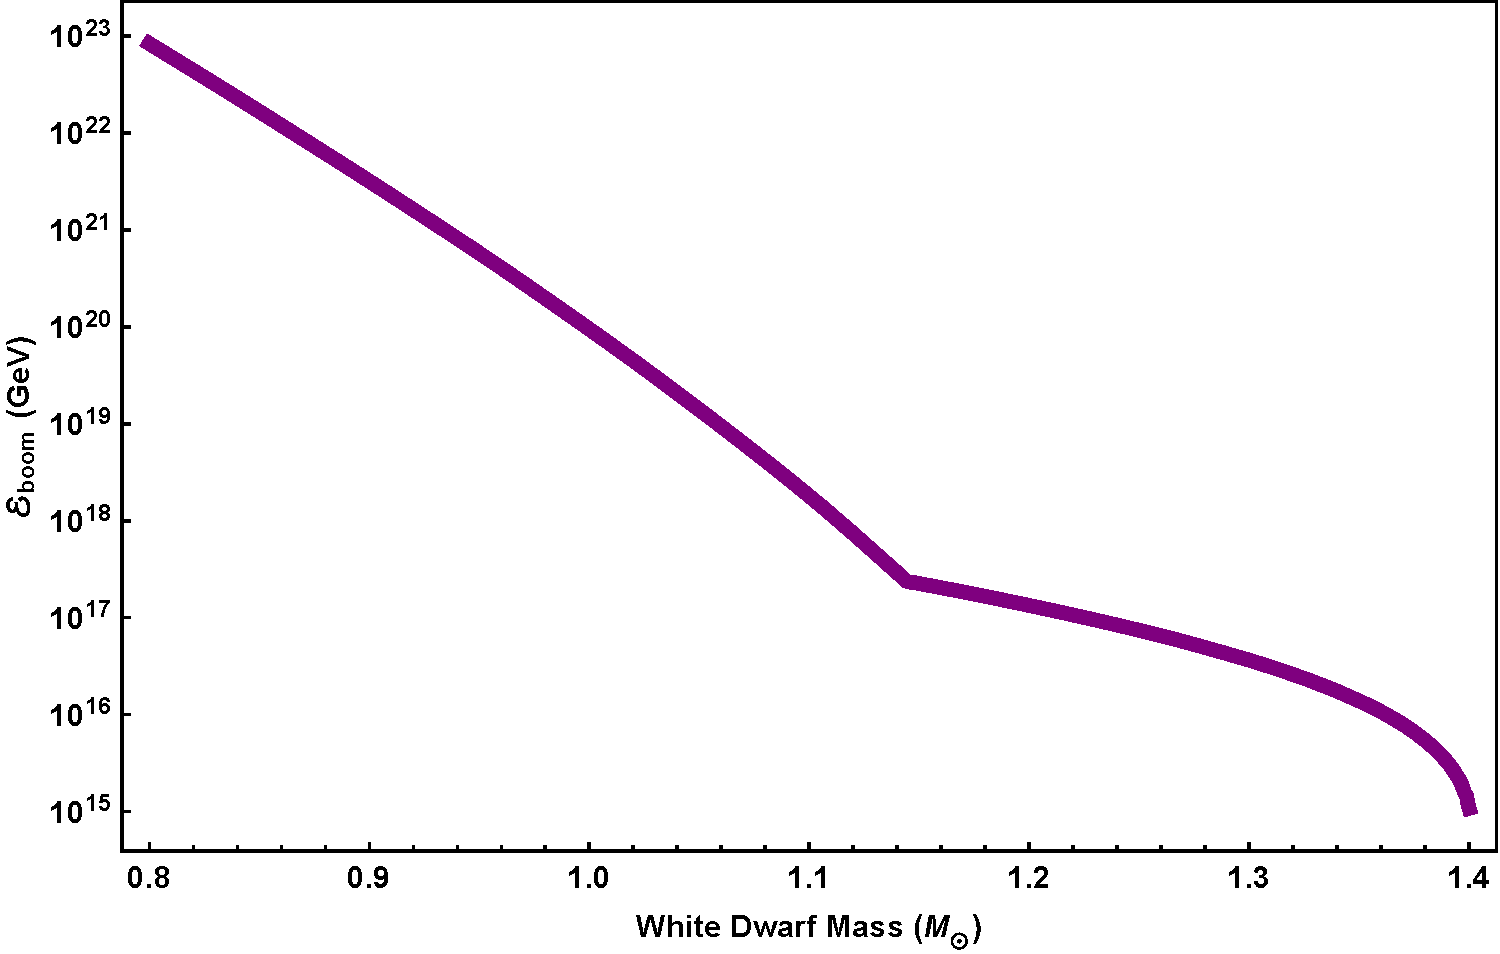
\includegraphics[scale=.35]{Eboom.pdf}
\caption{The minimum energy deposit~\eqref{eq:Eboom} necessary to trigger runaway fusion, based on numerical results for $\lambda_T$~\cite{Woosley} and the WD mass-density relation~\cite{cococubed}}.
\label{fig:Eboom}
\end{figure}
